% Fix citations
In this chapter, we perform simulations to gauge the effectiveness of the
DSD metric in improving the prediction of labels on data for scale-free
networks~\cite{PhysRevLett.90.058701}, Watts-Strogatz small-world
networks~\cite{Watts1998Collective}, and some networks we constructed with
hypotheses of how the DSD metric should affect classification on them. We 
compare the DSD metric with the shortest-path distance metric, which is 
used in some modern approaches of label prediction, such as k-nearest 
neighbor classifiers~\cite{10.1371/journal.pone.0076339} and laplacian 
eigenmaps~\cite{belkin2002laplacian}. Although several methods for 
measuring distance or similarity among vertices in a network use the 
shortest-path distance in the network, the DSD metric is designed to 
capture distinctions in similarity not captured by the shortest-path 
distance alone. Thus, we compare effectiveness of the DSD metric and the 
shortest-path distance metric. We expect the shortest path distance metric 
to be less effective than the DSD metric for networks with high clustering 
coefficients or networks with a small diameter, such as small-world 
networks. Any vertex in such a network is close to any other node in the 
network, making the shortest-path distance of any two nodes close. We also 
expect the DSD metric to be more effective on networks with hub vertices, 
since these vertices tend to make the network highly connected with a small 
diameter.

% Change this to say something about resistance distance instead of centrality
In the same way, we compare the DSD metric with resistance distance.

We hope to reveal properties of graphs that allow the DSD metric to be more 
effective at classification.


\section{Noisy Complete Components (NCC) Graphs}
In this section, we construct NCC graphs and run simulations on these 
graphs to determine the effectiveness of different label prediction methods 
on these graphs. These graphs were chosen because they can be constructed 
with an intuitive binary labeling of vertices; NCC graphs are constructed 
from two complete graphs as defined in Chapter 3 Definition 18.

\subsection{Data Collection}
We studied the classification problem on the complete components graph. After constructing the complete components graph $G$ with parameters $n$, $p$ and $q$ described in the section above, we censored a proportion $censorP$ of the labels in $G$. We then used the weighted majority voting algorithm using $k$-nearest neighbors with respect to both the shortest path distance metric and the DSD metric to predict labels. To make sure the prediction accuracy was robust, we ran this process several times and took the average of the resulting prediction accuracies. We adding a parameter called $avgRuns$ to describe how many times we would run this process for the average prediction accuracy.

To test the behavior of the prediction accuracy with respect to different parameters of the complete components graph, we ran several simulations using varying parameter inputs. The parameter $n$, the size of one complete graph used in the construction of the complete components graph, was set to $250$. A constant value for this parameter sufficiently large would allow us to observe differences in prediction accuracy and changing this parameter would not affect the prediction accuracy. The parameter for the average number of runs for calculating prediction accuracy, $avgRuns$ was also set to a constant value of $10$, since this parameter would not affect the prediction accuracy. The parameter for the proportion of the graph labels to censor, $censorP$, was also set to a constant $0.3$ because this would not affect the prediction accuracy, as shown in figure \ref{fig:censor_param}.

% Hard to read
\begin{figure}[h!]
\centering
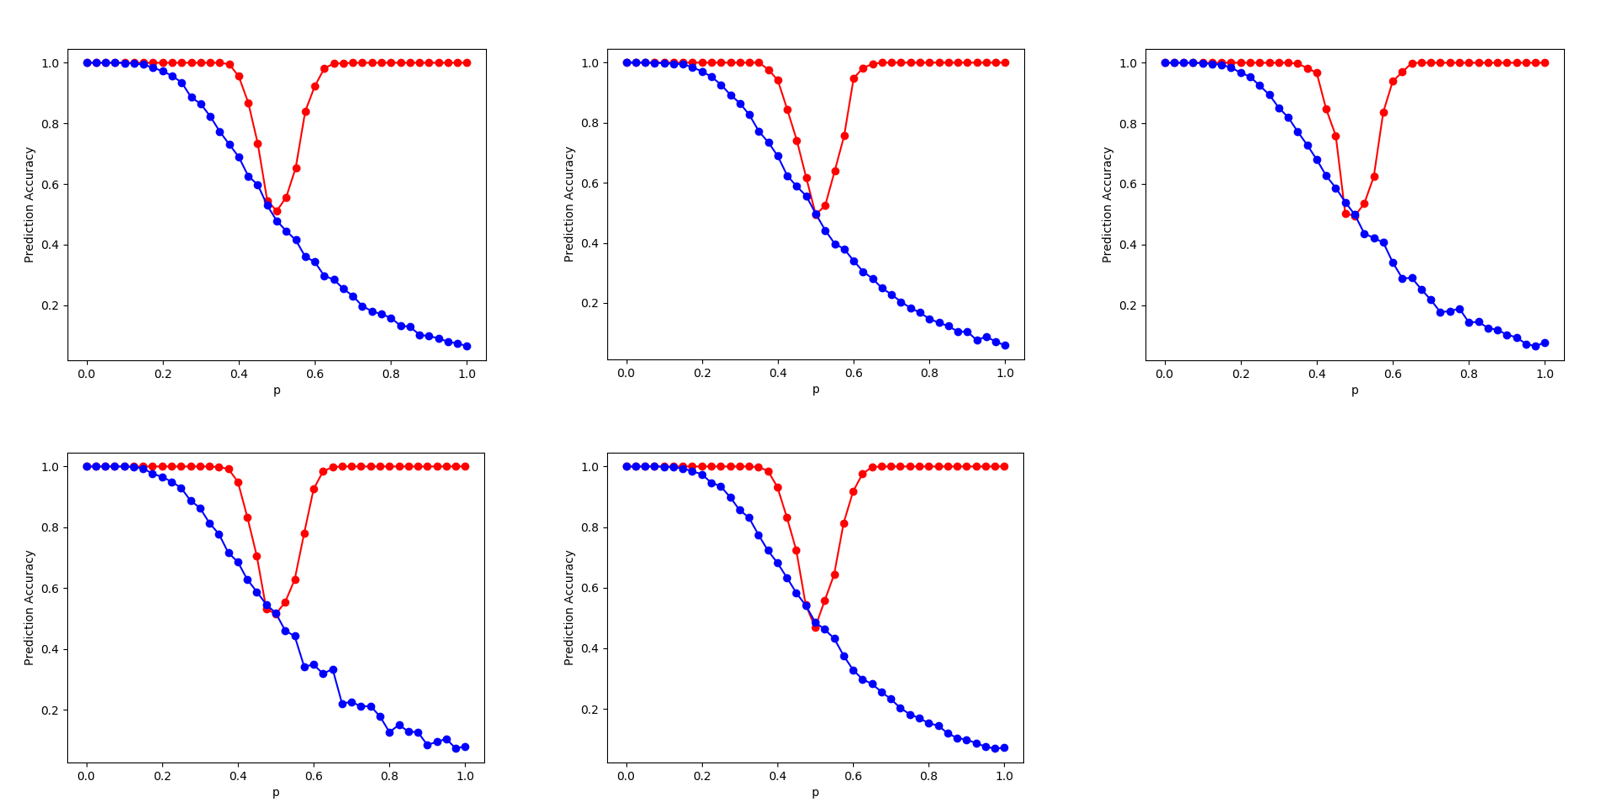
\includegraphics[width=1.0\textwidth]{censor_param.png}
\caption{Plots showing that the censoring parameter $censorP$ has no affect on prediction accuracy. $n = 250$, $avgRuns = 10$, $q = 0.5$, $p$ goes from $0$ to $1$ in intervals of $0.025$, and $censorP$ goes from $0.1$ to $0.9$ in intervals of $0.2$.}
\label{fig:censor_param}
\end{figure}


The parameters that we varied in our simulations for the complete components graphs were $p$ and $q$. Figure \ref{fig:cc_p_q} shows a plot of prediction accuracies for a fixed $q = 0.5$ and $p$ going from $0$ to $1$ in intervals of $0.025$. Figure \ref{fig:cc_q_p} shows a plot of prediction accuracies for a fixed $p = 0.5$ and $q$ going from $0$ to $1$ in intervals of $0.025$.

\begin{figure}[h!]
\centering
\includegraphics[width=0.75\textwidth]{{cc_p_n250_q0.5_c0.1_avg10_mv-k20}.png}
\caption{A plot showing the change in prediction accuracy for a fixed $q = 0.5$ and $p$ from $0$ to $1$ in intervals of $0.025$.}
\label{fig:cc_p_q}
\end{figure}

\begin{figure}[h!]
\centering
\includegraphics[width=0.75\textwidth]{{cc_q_n250_p0.5_c0.1_avg10_mv-k20}.png}
\caption{A plot showing the change in prediction accuracy for a fixed $p = 0.5$ and $q$ from $0$ to $1$ in intervals of $0.025$.}
\label{fig:cc_q_p}
\end{figure}


\subsection{Analysis}
We can expect prediction using the DSD metric to do significantly better than prediction using the shortest path distance metric as described below. Figure \ref{fig:cc_p_q} and Figure \ref{fig:cc_q_p} show this using expected values.

Using the parameters from the simulation run shown in Figure \ref{fig:cc_p_q}, we get that for an arbitrary vertex $v$, $deg_{same}(v) = (1-0.5)(250-1) = 124.5$. Since $deg_{diff} = 250p$, we know that $deg_{diff}$ will increase or decrease proportional to the change in $p$. For values of $p$ between $0$ and $0.5$, we know that $deg_{same} > deg_{diff}$. It is clear that the shortest path distance metric should predict with a fairly high accuracy for $p$ close to $0$, but should predict no better than a random guess for $p$ close to $0.5$. The prediction accuracy of the shortest path distance only becomes worse for $p$ greater than $0.5$, since $deg_{same} < deg_{diff}$.

\section{Noisy Complete Components with Hubs (NCCH) Graphs}
We studied NCCH graphs in order to determine the effects of hub vertices on the prediction accuracies of NCC graphs. The graphs used were chosen with similar parameters from the NCC graphs in order to compare results. The NCCH graphs were also constructed with an intuitive binary labeling of vertices with hub vertices labeled randomly.
\subsection{Data Collection}
We used the same values for similar parameters to the NCC graphs as described in the previous sections. The same values for the parameters $n$,$avgRuns$, and $censorP$ were used. The same process of fixing the parameter $p$ while varying the parameter $q$ and fixing $q$ while varying $p$ was used.

\begin{figure}[h!]
\centering
\includegraphics[width=0.75\textwidth]{{NCCH_fix_q}.png}
\caption{A plot showing the change in prediction accuracy for a fixed $q = 0.5$ and $p$ from $0$ to $1$ in intervals of $0.025$.}
\label{fig:NCCH_fix_q}
\end{figure}

\begin{figure}[h!]
\centering
\includegraphics[width=0.75\textwidth]{{NCCH_fix_p}.png}
\caption{A plot showing the change in prediction accuracy for a fixed $p = 0.5$ and $q$ from $0$ to $1$ in intervals of $0.025$.}
\label{fig:NCC_fix_p}
\end{figure}
\subsection{Analysis}

\section{Class-weighted Barab\'{a}si-Albert (CWBA) Graphs}
\subsection{Data Collection}
\subsection{Analysis}